\documentclass{beamer}
%
% Choose how your presentation looks.
%
% For more themes, color themes and font themes, see:
% http://deic.uab.es/~iblanes/beamer_gallery/index_by_theme.html
%
\mode<presentation>
{
  \usetheme{Madrid}      % or try Darmstadt, Madrid, Warsaw, ...
  \usecolortheme{default} % or try albatross, beaver, crane, ...
  \usefonttheme{default}  % or try serif, structurebold, ...
  \setbeamertemplate{navigation symbols}{}
  \setbeamertemplate{caption}[numbered]
} 

\usepackage[english]{babel}
\usepackage[utf8x]{inputenc}
\usepackage{listings}

\title[\LaTeX intro]{A short introduction to \LaTeX}
\author{Teacher name}
\institute{LinuxUPC}
\date{\today}

\begin{document}

\begin{frame}
  \titlepage
\end{frame}


\begin{frame}{Outline}
  \tableofcontents
\end{frame}

\section{Introduction}

\begin{frame}{Introduction}

\begin{itemize}
  \item What is \LaTeX?
  \item Who invented it?
\end{itemize}
\begin{figure}
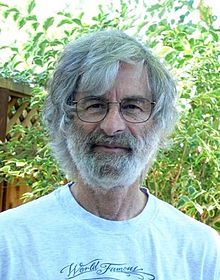
\includegraphics[width=0.35\textwidth]{graphics/author.jpg}
\caption{\label{fig:latexCreator}{Leslie Lamport, \LaTeX original author}}
\end{figure}

\vskip 1cm
%\begin{block}{Examples}
%Block block block template
%\end{block}
\end{frame}

\section{Installation}

\begin{frame}{Installtion}
Shall I install \LaTeX?
\begin{itemize}
    \item Are you comfortable with your text editor and it supports latex snippets and you love configuring things? Then yes.
    \item You want to write documents collaboratively, don't install things and have a working environment? Then use overleaf.
\end{itemize}
\end{frame}
\begin{frame}{Overleaf}
Overleaf is a web \LaTeX editor with a lot of features, it's awesome!
\begin{figure}
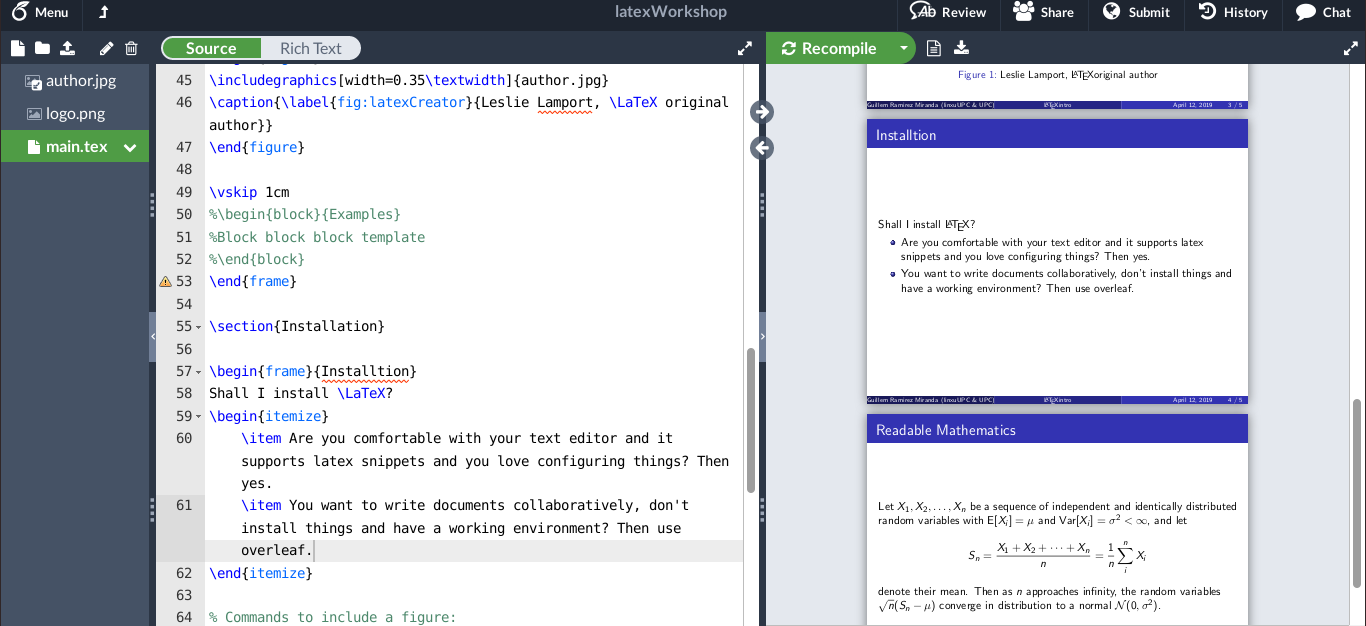
\includegraphics[width=0.75\textwidth]{graphics/overleaf.png}
\caption{\label{fig:overleaf}{Overleaf capture}}
\end{figure}
% Commands to include a figure:
%\begin{figure}
%\includegraphics[width=\textwidth]{your-figure's-file-name}
%\caption{\label{fig:your-figure}Caption goes here.}
%\end{figure}

\end{frame}
\begin{frame}{Custom environment}
Or you can install a \LaTeX compiler, and use your desired editor. 
\begin{figure}
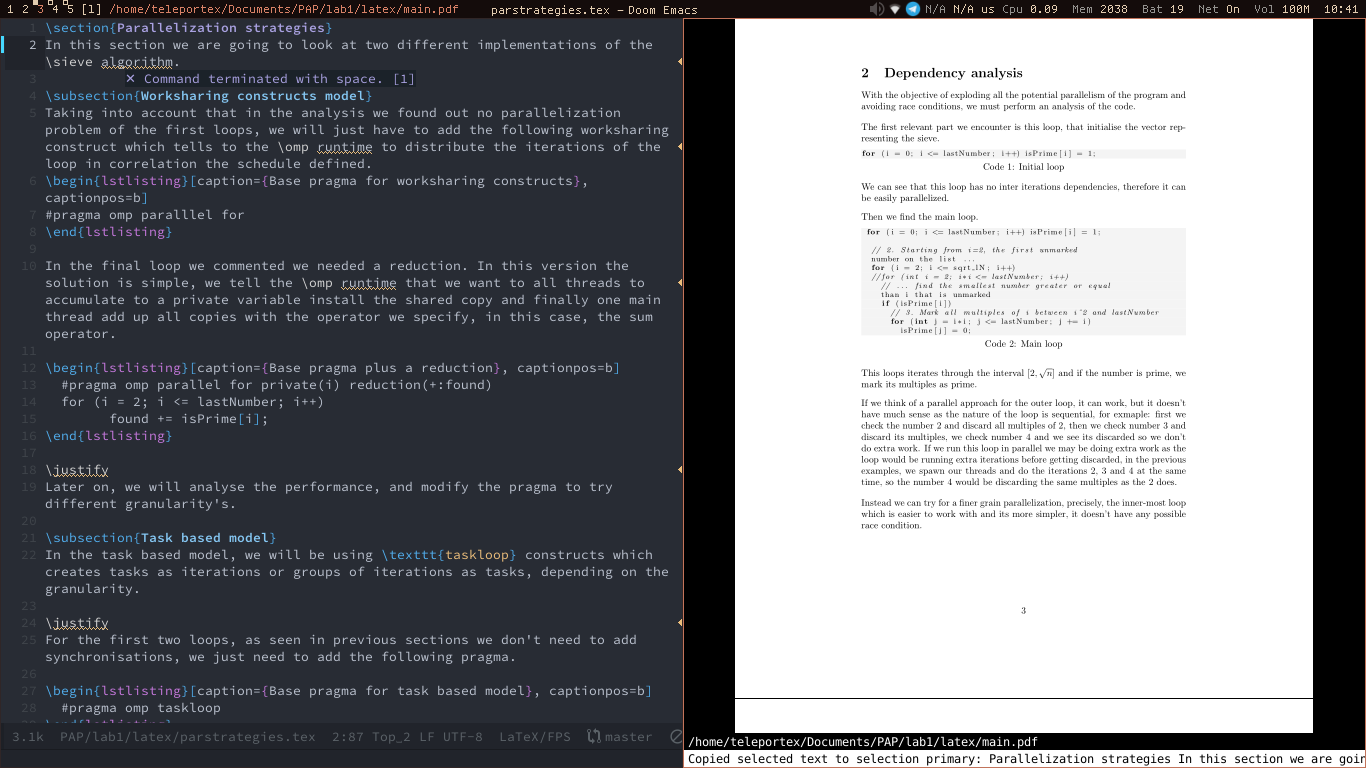
\includegraphics[width=0.75\textwidth]{graphics/custom.png}
\caption{\label{fig:custom}{My custom environment capture}}
\end{figure}

\end{frame}

\section{Your first document}

\begin{frame}[fragile]{\LaTeX basic layout}
This is the basic latex layout
\begin{lstlisting}[language=]
\documentclass{article}
\begin{document}
  Hello World!
\end{document}
\end{lstlisting}

\end{frame} 

\end{document}